% \section{The reciprocal theorem and equaitons for a droplet force and Stresslet}
% \label{ap:reciprocal}
\section{Introduction}


We revisit the methodology of \citet{stone2001inertial,raja2010inertial,dabade2015}  to compute the first moment of force on a spherical droplet embedded in a uniform flow at low but finite inertia effects. 
In opposition to \citet{stone2001inertial} and \citet{raja2010inertial} who considered neutrally-buoyant sherical inclusion embedded in a shear flow, we focus on the relative motions of droplets with the continuous phase. 
\citet{dabade2015} computed the torque (skew-symmetric part of the first moment) on a spheroidal particle embedded in a uniform flow. 
Our study is similar to the work of \citet{dabade2015}, however we aim to compute the whole first moment tensor (not only the torque), and we consider droplets (instead of solid spheroidal particles). 
Therefore, we propose an original method, mainly inspired from \citet{stone2001inertial}, to compute the first moment of force on droplets at first order $Re$.  



\section{Problem and governing equations}
We consider a dilute emulsion of spherical droplets at low but finite inertial effects. 
In this situation, we have shown that the relevant equations to be solved to compute the closure terms of the averaged equations are the disturbance fields equations, or the conditionally-averaged equations \citep{fintzi2025}. 
For ease of notation we note here $\textbf{u}_k$ the disturbance fields generated by a spherical droplet.  
The indice $k$ denotes either the dispersed phase $k = d$ or the continuous phase $k=f$. 
$\textbf{u}_k$ is conditioned on the presence of a droplet at \textbf{y} with center of mass velocity \textbf{w}.
The ensemble-averaged velocity or ``background flow'' velocity, is written $\textbf{U}_f[\textbf{x},t]$. 
In this case $\textbf{u}_k[\textbf{x}|\textbf{y},\textbf{w}] + \textbf{U}_f[\textbf{x}]$ represents the velocity field seen by an observer in the laboratory frame of reference .
Note that the averaged velocity or ``background flow'' velocity field $\textbf{U}_f[\textbf{x},t]$ can be re-written in terms of a Taylor series expansion around the particle center of mass such that, $\textbf{U}_f[\textbf{x}] = \textbf{U}_f[\textbf{y}] + \textbf{r} \cdot \grad \textbf{U}_f|_{\textbf{x} =\textbf{y}} + \ldots$. 
On \ref{fig:disturbance} we display a schematic representation of the problem. 
\begin{figure}
    \centering
    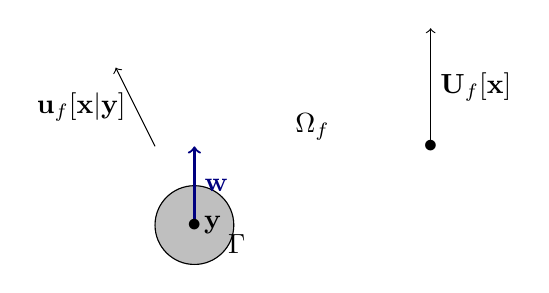
\begin{tikzpicture}
        \filldraw[ gray!50!white](0,0)circle (0.5);
        \draw(0,0)circle (0.5)node[right,below]{   $\;\;\;\;\;\;\;\;\;\;\;\Gamma$};
        \draw[->,blue!50!black,thick](0,0)--++(0,1)node[midway,right]{$\textbf{w}$};
        \draw (0,0)node{$\bullet$}node[right]{$\textbf{y}$};
        \draw[->](-0.5,1)--++(-0.5,1)node[midway,left]{$\textbf{u}_f[\textbf{x}|\textbf{y}]$};
        \draw[->] (3,1)node{$\bullet$}--++(0,1.5)node[right,midway]{$\textbf{U}_f[\textbf{x}]$};
        \draw (1.5,1.25)node{$\Omega_f$};
    \end{tikzpicture} 
    \caption{Representation of the problem parameters.}
    \label{fig:disturbance}
\end{figure}
Out of the volume of the droplet centered at \textbf{y}, we may write the single-particle conditionally averaged Navier-Stokes equations as,  
\begin{align*}
    \div\bm\sigma_f
    &= 
    Re [
    \pddt \textbf{u}_f
    + \textbf{u}_f\cdot \grad \textbf{u}_f
    + \textbf{u}_f\cdot \grad (\textbf{U}_f - \textbf{w})
    + (\textbf{U}_f - \textbf{w})\cdot \grad \textbf{u}_f]\\
    &= Re \textbf{f}_f\\
    \div \textbf{u}_f &= 0
\end{align*}
and, 
\begin{align*}
    \div\bm\sigma_d
    &= 
    \frac{\zeta}{\lambda}Re [
    \pddt \textbf{u}_d
    + \textbf{u}_d\cdot \grad \textbf{u}_d
    + \textbf{u}_d\cdot \grad (\textbf{U}_f - \textbf{w})
    + (\textbf{U}_f - \textbf{w})\cdot \grad \textbf{u}_d]\\
    &= \frac{\zeta}{\lambda}Re \textbf{f}_d\\
    \div \textbf{u}_d &= 0,
\end{align*}
%in the domain of the droplet centered at $\textbf{y}$. 
where, $\bm\sigma_{k} = -p_{k}\bm\delta + (\grad \textbf{u}_{k} + \grad \textbf{u}_{k}^{\text{t}})$ is the dimensionless disturbance stress, with $p_k$ the disturbance pressure field. 
We introduce the Reynolds number $Re = \frac{\rho_f a U}{\mu_f}$ which is based on the droplet radius $a$, the density ratio $\zeta = \rho_d / \rho_f$ and the viscosity ratio $\lambda = \mu_d / \mu_f$ , with $U = |\textbf{U}_f[\textbf{y}] - \textbf{w}|$. 
Note that the distances have been made dimensionless using the droplet radius $a$. 
The boundary conditions at the droplet surface ($i.e. |\textbf{r}| = |\textbf{x} - \textbf{y}| = 1$) are, 
\begin{align}
    \textbf{n}\cdot\textbf{u}_f
    &= \{\textbf{w} - \textbf{U}_f[\textbf{x},t]\}\cdot \textbf{n} 
    = \textbf{U}[\textbf{x},t]\cdot \textbf{n} \\
    \textbf{u}_f &= \textbf{u}_d\\
    (\bm\sigma_f\cdot\textbf{n})\cdot (\bm\delta - \textbf{nn})
    &= \lambda (\bm\sigma_d\cdot \textbf{n})\cdot (\bm\delta - \textbf{nn}),
    \label{eq:bc_stress_orig}
\end{align}
where we have introduced the relative velocity field $\textbf{U}[\textbf{x},t] = \textbf{w} - \textbf{U}_f[\textbf{x},t]$. 
These boundary conditions are completed by the following boundary conditions far from the droplet,
\begin{align*}
    \lim_{|\textbf{r}|\to\infty }\textbf{u}_f[\textbf{x}|\textbf{y}] = 0,\\
    \lim_{|\textbf{r}|\to\infty }p_f[\textbf{x}|\textbf{y}] = 0. 
\end{align*}

\section{Regular expansion in $Re$} %for low but finite inertial flows}

To simplify the problem we now consider small \textit{Reynolds} numbers perturbations. 
When performing such an expansion methods one must usually consider an ``outer'' region and and an ``inner'' region \citet{proudman1957expansions}. 
% However, as shown in \citet{masoud2019reciprocal} the ``outer'' solution provides only an $\mathcal{O}(Re^{3/2})$ on the closure terms of interest in our work.
%However, as shown in \citet{leal1980, stone2001inertial,raja2010inertial,dabade2015} we may disregard the ``outer'' solution and only focus on the ``inner'' expansion for certain problem for which the outer solution does not contribute to the leading order to the volume integral involved in the reciprocal theorem.
% obtaining a result accurate at $\mathcal{O}(Re)$. 
As demonstrated in \citet{leal1980, stone2001inertial, raja2010inertial, dabade2015}, we can disregard the "outer" solution and concentrate solely on the "inner" expansion for specific problems where the outer solution does not contribute to the leading-order term of the volume integral involved in the reciprocal theorem.
Here we aim to compute the first moment of the hydrodynamic forces and not the drag force on the droplet (which requires the outer expansion \citep{proudman1957expansions}). 
More details will be given below. %for instance just retain, that only a regular expansion in $Re$ is necessary.

The disturbance velocity field of phase $k$ may be re-written as an expansion around $Re \approx 0$ namely, 
\begin{equation*}
    \textbf{u}_k = \textbf{u}_k^{(0)} + Re \textbf{u}_k^{(1)} + \ldots
\end{equation*}
with similar expression for the fields $\bm\sigma_k$ and $\textbf{f}_k$. 
Substituting these expansions into the governing equations gives,
\begin{align}
    \div\bm\sigma_f^{(0)}
    = 0,
    && \div \textbf{u}_f^{(0)} = 0 
    \label{eq:zeroth_order_NS_f}
    \\
    \div\bm\sigma_f^{(1)},
    =  \textbf{f}_f^{(0)},
    && \div \textbf{u}_f^{(1)} = 0.  
    \label{eq:first_order_NS_f}
\end{align}
While in the dispersed phase we obtain, 
\begin{align}
    \div\bm\sigma_d^{(0)}
    = 0,
    && \div \textbf{u}_d^{(0)} = 0 
    \label{eq:zeroth_order_NS_d}
    \\
    \div\bm\sigma_d^{(1)},
    = \frac{\zeta}{\lambda} \textbf{f}_d^{(0)},
    && \div \textbf{u}_d^{(1)} = 0. 
    \label{eq:first_order_NS_f}
\end{align}
Where we truncated the expansion at $\mathcal{O}(Re)$.  
The boundary conditions can also be written as, 
\begin{align}
    \textbf{n}\cdot\textbf{u}_f^{(0)}
    &= \textbf{U}[\textbf{x},t]\cdot \textbf{n} \\
    \textbf{n}\cdot\textbf{u}_f^{(1)}
    \label{eq:bc_inertia_u}
    &= 0, \\
    \label{eq:bc_non_inertia}
    (\bm\sigma_f^{(0)}\cdot\textbf{n})\cdot (\bm\delta - \textbf{nn})
    &= \lambda (\bm\sigma_d^{(0)}\cdot \textbf{n})\cdot (\bm\delta - \textbf{nn}),\\
    (\bm\sigma_f^{(1)}\cdot\textbf{n})\cdot (\bm\delta - \textbf{nn})
    &= \lambda (\bm\sigma_d^{(1)}\cdot \textbf{n})\cdot (\bm\delta - \textbf{nn}). 
    \label{eq:bc_inertial}
\end{align}


\section{Tests solution}

The Reciprocal theorem requires the use of a known solution.
We call that solution the \textit{test} solution, since its only purpose is to compute the \textit{real} solution of the equations introduced above. 
We note the test velocity and stress fields $\hat{\textbf{u}}_k$ and $\hat{\bm\sigma}_k$, respectively. 
We consider two tests problem.
\subsection{Stokes flow solution for a droplet embedded in uniform and shear flow}
\begin{align}
    \div \hat{\textbf{u}}_k = 0 
    && \div \hat{\bm\sigma}_k = 0 
    \label{eq:test_sol}
\end{align}
in phase $k$ and, 
\begin{align}    
    \textbf{n}\cdot \hat{\textbf{u}} &=  \textbf{n}\cdot \hat{\textbf{U}}[\textbf{x}] = \textbf{n}\cdot \hat{\textbf{U}} - \textbf{r}\cdot \hat{\textbf{E}} \cdot \textbf{n}\\
    \hat{\textbf{u}_f} &= \hat{\textbf{u}_d}\\
    (\hat{\bm\sigma_f}\cdot \textbf{n}) \cdot (\bm\delta - \textbf{nn})
    &= 
    \lambda (\hat{\bm\sigma_d}\cdot \textbf{n}) \cdot (\bm\delta - \textbf{nn}) \label{eq:bc_stress}
\end{align} 
on the interface of the droplet centered at the origin. 
Furthermore, we note $\hat{\textbf{U}} = \textbf{w} - \hat{\textbf{U}}_f$, with $\hat{\textbf{U}}_f$ a linear with $\textbf{r}$ such that $ \hat{\textbf{U}}_f[\textbf{x}] = \hat{\textbf{U}}_f[\textbf{y}]+\textbf{r}\cdot \hat{\textbf{E}}[\textbf{y}]$  where \textbf{x} is the position of the droplet center of mass and \textbf{y} a point in the domain.
Note that $\hat{\textbf{U}}$ and $\hat{\textbf{U}}_f$ are both linear function of position, i.e. we do not consider quadratic background velocity for the ``test''  problem. 

This problem has been treated extensively in the literature, \citet{pozrikidis1992boundary,leal2007advanced,kim2013microhydrodynamics}, the solutions read, 
\begin{align}
    \hat{\textbf{u}}_k = \mathcal{U}_k\cdot \hat{\textbf{U}}+ \mathcal{E}_k : \hat{\textbf{E}}\\
    \hat{p}_k = \mathcal{U}_k^p\cdot \hat{\textbf{U}}+ \mathcal{E}_k^p : \hat{\textbf{E}}\\
    \hat{\textbf{e}}_k = \mathcal{U}_k^e\cdot \hat{\textbf{U}}+ \mathcal{E}_k^e : \hat{\textbf{E}}\\
    \hat{\bm\sigma}_k = \mathcal{U}_k^\sigma\cdot \hat{\textbf{U}}+ \mathcal{E}_k^\sigma : \hat{\textbf{E}}
    \label{eq:solution_hat}
\end{align}
with, 
\begin{align*}
    (\mathcal{U}_{f})_{ik} &= 
    % \delta_{ik}
     \frac{1}{4}\left(\frac{3\lambda + 2}{\lambda +1}\right)
    \left(\frac{\delta_{ik}}{r} + \frac{r_ir_k}{r^3}\right) 
    + 
    \frac{1}{4}\left(\frac{\lambda}{\lambda +1}\right)
    \left(\frac{\delta_{ik}}{r^3} - \frac{3r_ir_k}{r^5}\right)  \\
    (\mathcal{E}_{f})_{ijk}
    &=
    %  \bm\delta\textbf{r}
    -\frac{\lambda}{(\lambda + 1)r^5} \delta_{ij} r_k
    -\left(
        5\lambda +2
        - \frac{5\lambda}{r^2}
        \right) 
    \frac{r_ir_jr_k}{2(\lambda+1)r^5}\\
    (\mathcal{U}_{d})_{ik} &= 
    \frac{1}{2}\left(\frac{2\lambda +3}{\lambda +1}\right)\delta_{ij}
    -\frac{1}{2} (2r^2 \delta_{ij} - r_ir_j)
    \left(\frac{1}{\lambda +1}\right)\\
    (\mathcal{E}_{d})_{ijk}
    &= -\delta_{ij} r_k
    + \frac{5r^2 -3}{2(\lambda +1)} \delta_{ij} r_k
    - \frac{1}{\lambda+1}r_ir_jr_k\\
    (\mathcal{U}_f^p)_i &= 
      \frac{1}{2}\left(\frac{3\lambda + 2}{\lambda +1}\right) \frac{r_i}{r^3}\\
     (\mathcal{U}_d^p)_i &= 
    - 5 \left(\frac{1}{\lambda +1}\right) r_i\\
    (\mathcal{E}_f^p)_{ij} &= - \frac{(5\lambda+2)}{(\lambda+1)r^5}r_ir_j\\
    (\mathcal{E}_d^p)_{ij} &= \frac{21\lambda}{2(\lambda+1)} r_ir_j\\
    (\mathcal{U}_k^e)_{ijk}
    &= 
    \frac{1}{2}(
    \partial_j 
    \mathcal{U}_{f,ik}
    + 
    \partial_i 
    \mathcal{U}_{f,jk}
    )\\
    (\mathcal{E}_k^e)_{ijkl}
    &= 
    \frac{1}{2}(
    \partial_j 
    \mathcal{E}_{f,ikl}
    + 
    \partial_i 
    \mathcal{E}_{f,jkl}
    )\\
    (\mathcal{U}_k)_{ijk}^\sigma  n_j 
    &= 
     - (\mathcal{U}_k^p)_{k}\delta_{ij}
     + 2(\mathcal{U}_k^e)_{ijk}
     = - \frac{2}{\lambda +1}\left(
         \frac{3}{4}\lambda\delta_{ik} 
         + \frac{3}{2} n_in_k
     \right)
     \\
     (\mathcal{E}_k^\sigma)_{ijkl}
     &=
     - (\mathcal{E}_k^p)_{kl}\delta_{ij}
     + 2(\mathcal{E}_k)_{ijkl}
\end{align*}
Particularly, note the linearity of the velocity, pressure and stress fields with the relative velocity $\hat{\textbf{U}}$ and the shear rate $\hat{\textbf{E}}$. 
We also give the expression, 
\begin{equation*}
    (\mathcal{U}_d^e)_{ijk} 
    % = 
    % 3(-4\delta_{ik} r_j + \delta_{ij} r_k + \delta_{kj} r_i)
    % + 10 r_j  \delta_{ik}
    = 
    - \frac{1}{2\lambda}\left(\frac{1}{1+\lambda}\right)(-2 \delta_{ik} r_j + 3\delta_{ij} r_k + 3\delta_{kj} r_i) ,
\end{equation*}
which will be useful for the following. 

\subsection{Point source solution}
Following, \citet{stone2001inertial} we now use the test problem of a point source of strength $Q$ located at the center of the sphere, in this case the test velocity  and stress fields, reads, 
\begin{align}
    \hat{\textbf{u}}_f = \frac{Q}{4\pi} \frac{\textbf{r}}{r^3}
    && \hat{\bm\sigma}_f = \mu_f \frac{Q}{2\pi}\left(
        \frac{\bm\delta}{r^3}
        - \frac{3 \textbf{rr}}{r^5}
    \right)
    \label{eq:point_source}
\end{align}

\section{Reciprocal theorem} %at first order in Reynolds number}

To compute the first order correction in $Re$ we apply the same methodology as in \ref{app:faxen} where we compute the Faxen correction on droplets.% but on the first order equaitons. 
We start by deriving a relation for the domain outside the droplet.
By taking the dot product of \ref{eq:first_order_NS_f} with $\hat{\textbf{u}}_f$ and \ref{eq:test_sol} (with $k = f$) with $\textbf{u}_k^{(0)}$, and subtracting both expressions gives, 
\begin{equation*}
    \hat{\textbf{u}}_f\cdot \div\bm\sigma_f^{(1)}
    =
    \textbf{u}_f^{(1)} \cdot \div \hat{\bm\sigma}_f, 
    + \hat{\textbf{u}}_f\cdot  \textbf{f}^{(0)}_f
\end{equation*}
Carrying an integration on the exterior domain of the droplet, and using $\hat{\textbf{u}}_f =\hat{\textbf{u}}_f  - \hat{\textbf{U}} + \hat{\textbf{U}}$ gives, 
\begin{equation}
    \intS{\hat{\textbf{U}}\cdot  \bm\sigma_f^{(1)} \cdot \textbf{n}}
    + \intS{(\hat{\textbf{u}}_f - \hat{\textbf{U}})\cdot  \bm\sigma_f^{(1)} \cdot \textbf{n}}
    = 
    \intS{\textbf{u}_f^{(1)}\cdot  \hat{\bm\sigma}_f \cdot \textbf{n}}
    - \intOf{\hat{\textbf{u}}_f\cdot  \textbf{f}^{(0)}_f}
    % \intOf{\textbf{u}_f^{(0)}\cdot ( \div \hat{\bm\sigma}_f)}
    \label{eq:stepone}
\end{equation}
From \ref{eq:bc_inertial} we deduce that $\textbf{u}_f^{(1)} \cdot \textbf{n} = 0$, allowing us to directly use the boundary condition on $\hat{\bm\sigma}_f$ for the first integral on the right-hand side. 
We now derive the reciprocal theorem on the interior of the drop to substitute the second term on the left-hand side of \ref{eq:stepone}. 
We multiply \ref{eq:test_sol} (with $k = f$) with $\textbf{u}_d^{(1)}$ and \ref{eq:first_order_NS_f} by $(\hat{\textbf{u}}_d - \hat{\textbf{U}})$, subtracting both expressions gives
\begin{equation*}
     \div [\bm\sigma_d^{(1)} \cdot (\hat{\textbf{u}}_d - \hat{\textbf{U}})]
     +2 \textbf{e}_d^{(1)} : \grad \hat{\textbf{U}}
     =
     \div [\hat{\bm\sigma}_d \cdot \textbf{u}_d^{(1)}]
     + \frac{\zeta}{\lambda}(\hat{\textbf{u}}_d - \hat{\textbf{U}}) \cdot \textbf{f}_d^{(0)}
\end{equation*}
Integrating on the volume of the particle gives, 
\begin{equation}
    \intS{ (\hat{\textbf{u}}_d - \hat{\textbf{U}})\cdot \bm\sigma_d^{(1)} \cdot \textbf{n}}
    + 2 \intO{ \textbf{e}_d^{(1)} : \grad \hat{\textbf{U}} }
    =
    \intS{\textbf{u}_d^{(1)}\cdot\hat{\bm\sigma}_d \cdot \textbf{n}} 
    + \frac{\zeta}{\lambda} \intO{(\hat{\textbf{u}}_d - \hat{\textbf{U}}) \cdot \textbf{f}_d^{(0)}}
    \label{eq:reci_interior}
\end{equation}
Multiplying this equation by $\lambda$, using the boundary conditions  for the interface stress and velocity fields, and then subtracting it to \ref{eq:stepone} gives the first form of the Reciprocal theorem for the first order inertial correction on spherical droplets, namely,
\begin{equation}
    \intS{\hat{\textbf{U}}\cdot  \bm\sigma_f^{(1)} \cdot \textbf{n}}
    -\lambda 2 \intO{ \textbf{e}_d^{(1)} : \grad \hat{\textbf{U}} }
    % + \intS{(\hat{\textbf{u}}_f - \hat{\textbf{U}})\cdot  \bm\sigma_f^{(1)} \cdot \textbf{n}}
    = 
    - \zeta \intO{(\hat{\textbf{u}}_d - \hat{\textbf{U}}) \cdot \textbf{f}_d^{(0)}}
    - \intOf{\hat{\textbf{u}}_f\cdot  \textbf{f}^{(0)}_f}.
    % \intS{\textbf{u}_f^{(1)}\cdot  \hat{\bm\sigma}_f \cdot \textbf{n}}
    % \intOf{\textbf{u}_f^{(0)}\cdot ( \div \hat{\bm\sigma}_f)}
    \label{eq:reciprocal_f_one}
\end{equation}
As for the Stokes flow relations, we are constrained to obtain a formula for the interface stress minus the internal shear.
Thus, one cannot get an independent results either for the surface stress or the internal rate of strain of the droplet.  
It motivates us to derive the second formulation of the reciprocal theorem.

We start by noting that, 
\begin{equation}
    \intO{ 2\textbf{e}_d^{(1)} : \grad \hat{\textbf{U}} }
    =\intO{ \grad \textbf{u}_d^{(1)} : (\grad \hat{\textbf{U}} +^\dagger \grad \hat{\textbf{U}}) }
    =
    \intS{  \textbf{u}_d^{(1)} \cdot (\grad \hat{\textbf{U}} + ^\dagger\grad \hat{\textbf{U}})  \cdot \textbf{n}}
    % &=
    % \intS{  \textbf{U} \cdot (\grad \hat{\textbf{U}} + ^\dagger\grad \hat{\textbf{U}})  \cdot \textbf{n}}
    % + \intS{  (\textbf{u}_d^{(1)} - \textbf{U})\cdot (\grad \hat{\textbf{U}} + ^\dagger\grad \hat{\textbf{U}})  \cdot \textbf{n}}
    % -\intO{\textbf{u}_d^{(0)} \cdot \grad^2 \hat{\textbf{U}} }
\end{equation}
Again, we used the property $\grad\grad \hat{\textbf{U}} = 0$. 
Injecting this formula into \ref{eq:reci_interior} yields,
\begin{equation*}
    \intS{ (\hat{\textbf{u}}_d - \hat{\textbf{U}})\cdot \bm\sigma_d^{(1)} \cdot \textbf{n}}
    =
    \frac{\zeta}{\lambda} \intO{(\hat{\textbf{u}}_d - \hat{\textbf{U}}) \cdot \textbf{f}_d^{(0)}}
    % \intS{  \textbf{u}_d^{(1)} \cdot (\grad \hat{\textbf{U}} + ^\dagger\grad \hat{\textbf{U}})  \cdot \textbf{n}}
    + \intS{
         \textbf{u}_d^{(1)}\cdot[\hat{\bm\sigma}_d  - (\grad \hat{\textbf{U}} + ^\dagger\grad \hat{\textbf{U}})]\cdot \textbf{n}
    }
\end{equation*}
Multiplying this expression by $\lambda$, considering the boundary conditions \ref{eq:BCCCCCCCCCC3,eq:bc_inertial}, and subtracting the resulting expression to \ref{eq:stepone} gives,
\begin{equation}
    \intS{\hat{\textbf{U}}\cdot  \bm\sigma_f^{(1)} \cdot \textbf{n}}
    - \intO{
        2\textbf{e}_d^{(1)}:\grad \hat{\textbf{U}} 
   }
    = 
    - \zeta \intO{(\hat{\textbf{u}}_d - \hat{\textbf{U}}) \cdot \textbf{f}_d^{(0)}}
    - \intOf{\hat{\textbf{u}}_f\cdot  \textbf{f}^{(0)}_f}. 
    % \intOf{\textbf{u}_f^{(0)}\cdot ( \div \hat{\bm\sigma}_f)}
    \label{eq:reciprocal_f2_one}
\end{equation}
This equation is the one that will be used to compute the \textit{Stresslet} tensor. 
Note that subtracting \ref{eq:reciprocal_f_one} to \ref{eq:reciprocal_f2_one} yields, 
% Since $\lambda$ is an arbitrary constant we deduce that, 
\begin{equation}
    (1-\lambda)\intO{
        2\textbf{e}_d^{(1)}:\grad \hat{\textbf{U}} 
   }
    = 0. 
    \label{eq:shearrrrr}
\end{equation}
Recall that this relation is only valid when  $\hat{\textbf{U}}$ is at most a linear field, which is assumed here. 

\subsection{Computations of the inertial stresslet for a particle in pure translation}

To compute the first moment of force, for a droplet in translation we set $\hat{\textbf{U}} = - \textbf{r} \cdot \hat{\textbf{E}}_f$, and $\textbf{U}[\textbf{y}] = \textbf{U}[\textbf{x},t] = \textbf{w} - \textbf{U}_f[\textbf{y}]$. 
Injecting these expressions into \ref{eq:shearrrrr,eq:reciprocal_f2_one} leads us to
\begin{align}
    - \intO{
        2(\textbf{e}_d^{(1)})_{ij}
   }
    &= 0, \\
    \intS{r_i (\bm\sigma_f^{(1)} \cdot \textbf{n})_j}
    % -\lambda 2 \intO{ (\textbf{e}_d^{(1)})_{ij}  }
    &= 
    + \zeta\intO{(\mathcal{E}_d + \textbf{r}\bm\delta)_{ijk} (\textbf{f}_d^{(0)})_k }
    + \intOf{(\mathcal{E}_f )_{ijk}  (\textbf{f}^{(0)}_f)_k}
    \label{eq:stresslet}
\end{align}
Where it is implied that both side of the equation actually represents the symmetric traceless part of what is written.
These integrals require the calculation of integrals in terms of $\textbf{f}^{(0)}_k$. 
According to the definition of $\textbf{f}_k$ we may write, 
\begin{align}
    \label{eq:eq111}
    \zeta\intO{(\mathcal{E}_d + \textbf{r}\bm\delta)_{ijk} (\textbf{f}_d^{(0)})_k }
    &=
    \zeta\intO{(\mathcal{E}_d + \textbf{r}\bm\delta)_{ijk} 
    (
    \pddt \textbf{u}_f^{(0)}
    - \textbf{u}_f^{(0)} \cdot \grad \textbf{U}
    + (\textbf{u}_f^{(0)} - \textbf{U})\cdot \grad \textbf{u}_f^{(0)}
    )_k }\\
    \intOf{(\mathcal{E}_f )_{ijk}  (\textbf{f}^{(0)}_f)_k}
    &=
    \intOf{(\mathcal{E}_f )_{ijk}  
    (\pddt \textbf{u}_f^{(0)}
    - \textbf{u}_f^{(0)} \cdot \grad \textbf{U}
    + (\textbf{u}_f^{(0)} - \textbf{U})\cdot \grad \textbf{u}_f^{(0)}
    )_k}
    \label{eq:eq222}
\end{align}
Using symmetry arguments, and noting that  \textbf{U} is a uniform field, we may already remove the terms $\sim \pddt \textbf{u}^{(0)}_k$ and $\sim \grad \textbf{U}$ (i.e. the first two terms on the right-hand side of \ref{eq:eq222,eq:eq111}). 
Consequently, the expression that have to be computed read
\begin{align}
    \zeta\intO{(\mathcal{E}_d + \textbf{r}\bm\delta)_{ijk} (\textbf{f}_d^{(0)})_k }
    &=
    \zeta\intO{(\mathcal{E}_d + \textbf{r}\bm\delta)_{ijk} 
    ( (\textbf{u}_f^{(0)} - \textbf{U})\cdot \grad \textbf{u}_f^{(0)}
    )_k },
    \label{eq:eq111222}
    \\
    \intOf{(\mathcal{E}_f )_{ijk}  (\textbf{f}^{(0)}_f)_k}
    &=
    \intOf{(\mathcal{E}_f )_{ijk}  
    ((\textbf{u}_f^{(0)} - \textbf{U})\cdot \grad \textbf{u}_f^{(0)}
    )_k}. 
    \label{eq:eq222222222}
\end{align}
The velocity field $\textbf{u}_f^{(0)}$ satisfies the Stokes equations, hence one can use \ref{eq:solution_hat} and write $(\textbf{u}_f^{(0)})_k = (\mathcal{U}_k)_{ij}(\textbf{U})_j$ to compute the above integrals. 

Carrying the integration for  \ref{eq:eq111222} gives zero. 
The remaining integral \eqref{eq:eq222222222} can be computed and injected into \ref{eq:stresslet}, then taking the symmetric traceless part of the equation gives, 
\begin{multline}
    \frac{1}{2}\intS{(\bm\sigma_f^{(1)} \textbf{r} + \textbf{r} \bm\sigma_f^{(1)} -\frac{2}{3}(\textbf{r} \cdot \bm\sigma_f^{(1)} )\bm\delta)\cdot \textbf{n}}
    = \\
    - \frac{4\pi}{3}\frac{63 \lambda^{3} + 150 \lambda^{2} + 112 \lambda + 28}{80 \left(\lambda + 1\right)^{3}}
    [
        \textbf{UU} - \frac{1}{3}(\textbf{U}\cdot \textbf{U})\bm\delta 
    ]
\end{multline}
We deduce that the complete Stresslet term at $\mathcal{O}(Re)$ reads as, 
\begin{multline}
    \frac{1}{2}\intS{(\bm\sigma_f \textbf{r} + \textbf{r} \bm\sigma_f -\frac{2}{3}(\textbf{r} \cdot \bm\sigma_f )\bm\delta)\cdot \textbf{n}}
    = \\
    - Re \frac{4\pi}{3}\frac{63 \lambda^{3} + 150 \lambda^{2} + 112 \lambda + 28}{80 \left(\lambda + 1\right)^{3}}
    [
        \textbf{UU} - \frac{1}{3}(\textbf{U}\cdot \textbf{U})\bm\delta 
    ]
    + \mathcal{O}(Re^2)
    \label{eq:sol}
\end{multline}


% Therefore, at first order in $Re$ we obtain the dimensionless expression, 
% \begin{align}
%     \frac{1}{2}\pSavg{ (\bm\sigma_f \textbf{r} + \textbf{r} \bm\sigma_f -\frac{2}{3}(\textbf{r} \cdot \bm\sigma_f )\bm\delta) \cdot \textbf{n}}
%     % -\lambda 2 \intO{ (\textbf{e}_d^{(1)})_{ij}  }
%     % + \intS{(\hat{\textbf{u}}_f - \hat{\textbf{U}})\cdot  \bm\sigma_f^{(1)} \cdot \textbf{n}}
%     &= 
%     Re \phi C_1
%     [
%         \textbf{u}_{pf}^*\textbf{u}_{pf}^* - \frac{1}{3}(\textbf{u}_{pf}^*\cdot \textbf{u}_{pf}^*)\bm\delta 
%     ]\\
%     &+ Re \phi  C_1 
%     [
%         \pavg{\textbf{u}_\alpha'\textbf{u}_\alpha'}^* - \frac{2}{3}k_p^*\bm\delta 
%     ],\\
%     \label{eq:sol1} 
% \end{align}
% with, 
% \begin{equation}
%     C_1 = - \frac{63 \lambda^{3} + 150 \lambda^{2} + 112 \lambda + 28}{80 \left(\lambda + 1\right)^{3}}. 
% \end{equation}
% Where we have noted $\pavg{\textbf{u}_\alpha'\textbf{u}_\alpha'}^* = \pavg{\textbf{u}_\alpha'\textbf{u}_\alpha'}/(n_p U^2)$ and $k_p^* = k_p/U^2$. 
 

\subsection{Trace of the first moment}


Usin \ref{eq:point_source} solution in \ref{eq:stepone} gives, 
\begin{align*}
    \intS{ \textbf{r}\cdot  \bm\sigma_f^{(1)} \cdot \textbf{n}}
    = 
    \intS{\textbf{u}_f^{(1)} \cdot  \mu_f \frac{1}{2\pi}\left(
        \bm\delta
        - 3 \textbf{rr}
    \right) \cdot \textbf{n}}
    - \intOf{ \frac{\textbf{r}}{r^3}\cdot  \textbf{f}^{(0)}_f}
    = 
    - \intOf{ \frac{\textbf{r}}{r^3}\cdot  \textbf{f}^{(0)}_f}
\end{align*}
Since $\intS{\textbf{u}^{(1)} \cdot \textbf{n}} =0$ due to the divergence free property of $\textbf{u}^{(0)}$. 
Setting $\textbf{u}^{(0)} = \textbf{U}\cdot \mathcal{U}_f$, we obtain, 
\begin{equation}
    \intS{ \textbf{r}\cdot  \bm\sigma_f^{(1)} \cdot \textbf{n}}
    = \frac{4\pi}{3} \frac{3\lambda^2 + 6\lambda + 4}{16(\lambda +1 )^2} \textbf{U} \cdot \textbf{U}
\end{equation}
And more generally we have, 
\begin{equation}
    \intS{ \textbf{r}\cdot  \bm\sigma_f \cdot \textbf{n}}
    = Re \frac{4\pi}{3} \frac{3\lambda^2 + 6\lambda + 4}{16(\lambda +1 )^2} \textbf{U} \cdot \textbf{U}
    \label{eq:sol2} 
\end{equation}
% \begin{equation*}
%     \pSavg{ \textbf{r}\cdot  \bm\sigma_f^{(1)} \cdot \textbf{n}}
%     = \phi \frac{3\lambda^2 + 6\lambda + 4}{16(\lambda +1 )^2} (\textbf{u}_{pf}^* \cdot \textbf{u}_{pf}^*
%     + 2 k_p^*).
%     \label{eq:sol2} 
% \end{equation*}

\section{Discussion}
\subsection{Why the ``outer solution'' is negligible to leading order ?}

We end this study with some comments regarding the assumption of neglecting the outer field contribution in the first moment of the forces.
Our justification is similar to the one made in \citet{stone2001inertial,dabade2015}.  

In the general case (before any kind of Taylor expansions), we may compute the \textit{Stresslet} term based on the integral of $\mathcal{E}_f (\textbf{u}_f - \textbf{U})\grad \textbf{u}_f$ on the whole domain exterior to the drop. 
According to the singularity solution \eqref{eq:solution_hat} $\mathcal{O}((\textbf{u}_f - \textbf{U})\grad \textbf{u}_f \sim r^{-2})$, since $\textbf{U} \sim \mathcal{O}(1)$ and $\textbf{u}_f\sim \mathcal{O}(r^{-1})$. 
Likewise, $\mathcal{E}_f \sim r^{-2}$ hence $\mathcal{O}(\mathcal{E}_f (\textbf{u}_f - \textbf{U})\grad \textbf{u}_f) = r^{-4}$. 
Additionally, the outer solution domain range form $|\textbf{r}| > Re^{-1}$ to $|\textbf{r}|\to \infty$ for a droplet in translation \citep{proudman1957expansions}.
Consequently, the outer solution contribution to the first moment is given by\citep{stone2001inertial}, 
\begin{equation}
    \lim_{Re \to 0 }
    \int_{Re^{-1}}^\infty
    \mathcal{E}_f (\textbf{u}_f - \textbf{U})\grad \textbf{u}_f
    d\Omega
    =
    \lim_{Re \to 0 }
    \int_{Re^{-1}}^\infty
    \mathcal{O}(r^{-2})
    dr
    = \mathcal{O}(Re). 
\end{equation}
Since this term is already factor of $Re$ in the expression of the first moment we are allowed to neglect the outer field contribution. 
Consequently, \ref{eq:sol,eq:sol2} are accurate with an error of $\mathcal{O}(Re^2)$. 

\subsection{Conclusion}

For this study we conclude that: 
\begin{enumerate}
    \item 
    At finite inertial effects, a spherical droplet in translation possesses a non-null first moment of hydrodynamic forces, that is proportional to $\sim Re \textbf{UU}$ and $Re\sim \textbf{U}\cdot\textbf{U}$. 
    \item 
    %As first demonstrated by Einstein, the equivalent viscosity of a suspension in Stokes flow regime is obtained through the calculation of the Stresslet term. 
    The averaged first moment of forces on the surface of the droplets is, among other terms, a contribution to the effective stress of the emulsion. 
    Therefore, in the dilute regime, we may conclude that the effective stress of a non-buoyant emulsion is of the form $\sim Re \phi \textbf{UU}$ and $\sim Re \phi \textbf{U}\cdot \textbf{U}$ where $\phi$ is the volume fraction of droplets.
    Hence, relative motions between the droplets and the continuous phase induce the isotropic stresses given by \ref{eq:sol2} and deviatoric stresses given by \ref{eq:sol}. 
    %\item At finite inertial effects the spherical shape of a droplet in translation is not an equilibrium solution since the stresslet is non-zero. 
    %Hence, the results given by \ref{eq:sol,eq:sol2} constitute the first coefficient in a series expansion of small capillary numbers. 
    % Additionally, at first order in deformation we may show that the inertia matrix of the droplet is proportional to the stresslet term, we must conclude that the deformation $\sim Re \textbf{UU}$ as well. 
\end{enumerate}

\appendix

\section{Reciprocal theorem for droplets in Stokes flows}
\label{app:faxen}
We consider in a first step the reciprocal theorem applied to a situation where the ``real'' field also follow stokes equations such that $\textbf{u}_k =\textbf{u}_k^{(0)}$. 
This will enable us to compute the moments of forces on a droplet immersed in an arbitrary background velocity field $\textbf{U}_f$, i.e. the Faxen laws. 


\subsection{Continuous phase integral relation}

Let us take the dot product of \ref{eq:zeroth_order_NS_f} with $\hat{\textbf{u}}_f$ and \ref{eq:test_sol} (with $k = f$) with $\textbf{u}_k^{(0)}$, then subtracting both expressions gives, 
\begin{equation*}
    \hat{\textbf{u}}_f\cdot \div\bm\sigma_f^{(0)}
    =
    \textbf{u}_k^{(0)} \cdot \div \hat{\bm\sigma}_k, 
\end{equation*}
Upon integrating over $\Omega_f$ which is the domain outside the droplet at \textbf{y},  we obtain the following relation, 
\begin{equation*}
    \intS{\hat{\textbf{u}}_f\cdot  \bm\sigma_f^{(0)} \cdot \textbf{n}}
    % \intOf{\hat{\textbf{u}}_f\cdot  (\div \bm\sigma_f^{(0)})}
    = 
    \intS{\textbf{u}_f^{(0)}\cdot  \hat{\bm\sigma}_f \cdot \textbf{n}}
    % \intOf{\textbf{u}_f^{(0)}\cdot ( \div \hat{\bm\sigma}_f)}
\end{equation*}
We recall that $\Gamma_\alpha$ represents the domain of integration of the surface of the droplet. 
For solid particle $\textbf{u}_f^{(0)}$ is entirely determined by the no-slip boundary condition, hence this relation constitutes the basis to compute the stress distribution projected on the particle surface normal (which corresponds to the left-hand side term). 
However, note that for droplets the velocity fields $\textbf{u}_f^{(0)}$ is a priori unknown.
Therefore, we must use a ``tricks''. 
Using the identity $\textbf{u}_f = \textbf{u}_f +\textbf{U}_f-\textbf{U}_f$ we reformulate the reciprocal theorem as, 
\begin{equation}
    \intS{\hat{\textbf{U}}\cdot  \bm\sigma_f^{(0)} \cdot \textbf{n}}
    + \intS{(\hat{\textbf{u}}_f - \hat{\textbf{U}})\cdot  \bm\sigma_f^{(0)} \cdot \textbf{n}}
    = 
    \intS{\textbf{U}\cdot  \hat{\bm\sigma}_f \cdot \textbf{n}}
    + \intS{(\textbf{u}_f^{(0)} - \textbf{U})\cdot  \hat{\bm\sigma}_f \cdot \textbf{n}}
    \label{eq:reciprocal_f}
\end{equation}
The first integral on the left-hand side is the aim of this study (this represents the moments of forces), the other integrals remain to be calculated. 
% However, note that the unknown, $\bm\sigma_f^{(0)}$ appears on the  left-hand side of this equation. 
Then, note that both term $(\textbf{u}_f^{(0)} - \textbf{U})$ and $(\hat{\textbf{u}}_f - \hat{\textbf{U}})$ are by definition tangent vectors to the particle surface (i.e. vectors of the form $\sim (\bm\delta - \textbf{nn})$). 
Considering the boundary condition \ref{eq:bc_stress} and \ref{eq:bc_stress_orig} we deduce that $(\hat{\textbf{u}}_f - \hat{\textbf{U}})\cdot  \bm\sigma_f^{(0)} = \lambda (\hat{\textbf{u}}_d - \hat{\textbf{U}})\cdot  \bm\sigma_d^{(0)}$ and  $({\textbf{u}}_f^{(0)} - \hat{\textbf{U}})\cdot  \hat{\bm\sigma}_f = \lambda (\hat{\textbf{u}}_d^{(0)} - \hat{\textbf{U}})\cdot  \hat{\bm\sigma}_d$. 
To determine the stress within the droplet, we now use a reciprocal theorem within the droplet volume. 

\subsection{Dispersed phase integral relation}

We take the dot product of \ref{eq:zeroth_order_NS_d} with $\hat{\textbf{u}}_d - \hat{\textbf{U}}$ and \ref{eq:test_sol} (with $k=d$) with $\textbf{u}_d^{(0)} -\textbf{U}$, then subtracting both expressions gives, 
\begin{equation*}
    (\hat{\textbf{u}}_d - \hat{\textbf{U}})\cdot \div\bm\sigma_d^{(0)}
    =
    (\textbf{u}_d^{(0)} - \textbf{U}) \cdot \div \hat{\bm\sigma}_d, 
\end{equation*}
which can be reformulated as, 
\begin{equation*}
    \div [\bm\sigma_d^{(0)} \cdot (\hat{\textbf{u}}_d - \hat{\textbf{U}})]
    - \bm\sigma_d^{(0)} : \grad (\hat{\textbf{u}}_d - \hat{\textbf{U}})
    =
    \div [\hat{\bm\sigma}_d \cdot (\textbf{u}_d^{(0)} - \textbf{U})], 
    - \hat{\bm\sigma}_d : \grad ({\textbf{u}}_d^{(0)} - \textbf{U})
\end{equation*}
Noticing that $- \hat{\bm\sigma}_d : \grad ({\textbf{u}}_d^{(0)} - \textbf{U}) + \bm\sigma_d^{(0)} : \grad (\hat{\textbf{u}}_d - \hat{\textbf{U}}) = 2 \hat{\textbf{e}}_d : \grad \textbf{U} - 2 \textbf{e}_d^{(0)} : \grad \hat{\textbf{U}}$, 
(recall that $\hat{\textbf{e}}_d = (\grad \hat{\textbf{u}}_d + ^\dagger \grad \hat{\textbf{u}}_d)/2$ and ${\textbf{e}^{(0)}}_d = (\grad {\textbf{u}^{(0)}}_d + ^\dagger \grad {\textbf{u}^{(0)}}_d)/2$ ), and integrating over the volume of the particle yields, 
\begin{equation}
    \intS{(\hat{\textbf{u}}_d - \hat{\textbf{U}})\cdot \bm\sigma_d^{(0)} \cdot \textbf{n}}
    + 2\intO{\textbf{e}_d^{(0)} : \grad \hat{\textbf{U}}}
    =
    \intS{(\textbf{u}_d^{(0)} - \textbf{U}) \cdot  \hat{\bm\sigma}_d\cdot \textbf{n} }
    + 2\intO{\hat{\textbf{e}}_d : \grad \textbf{U}}. 
    \label{eq:reciprocal_d}
\end{equation}



\subsection{First form of the reciprocal theorem for stokes flows}

Making use of the relation \ref{eq:reciprocal_d} into \ref{eq:reciprocal_f} yields the first formulation of the reciprocal theorem for droplets, namely  
\begin{equation}
    \intS{\hat{\textbf{U}}\cdot  \bm\sigma_f^{(0)} \cdot \textbf{n}}
    - \lambda 2\intO{\textbf{e}_d^{(0)} : \grad \hat{\textbf{U}}}
    = 
    \intS{\textbf{U}\cdot  \hat{\bm\sigma}_f \cdot \textbf{n}}
    -\lambda  2\intO{\hat{\textbf{e}}_d : \grad \textbf{U}}. 
    \label{eq:reciprocal_all}
\end{equation}
As evidenced by the second term on the left-had side, this expression  allows one to compute the force traction (integral of $\bm\sigma_f^{(0)} \cdot \textbf{n}$) minus the internal shear of the droplet (integral of $\textbf{e}_d^{(0)}$) based on the test solution given by $\hat{\bm\sigma}_f$ and $\hat{\textbf{e}}_d$ (since the \textbf{U} will be related to the boundary conditions).
However, it is not possible to compute one of the terms independently of the other, i.e. either the integral of $\textbf{e}_d^{(0)}$ or the integral of $\bm\sigma_f^{(0)} \cdot \textbf{n}$. 
This introduces the need for a second formulation of the reciprocal theorem. 

\subsection{The second formulation of the reciprocal theorem}
The boundary condition of the stresses at the interface of the droplet is written,
\begin{equation}
    (\bm\sigma_f\cdot\textbf{n})\cdot (\bm\delta - \textbf{nn})
    = \lambda (\bm\sigma_d\cdot \textbf{n})\cdot (\bm\delta - \textbf{nn})
    \label{eq:BCCCCCCCCCC}
\end{equation}
Recall that $\bm\sigma_{f,d}$ are the disturbance stresses, i.e. they are computed based on the disturbance velocity fields: $\textbf{u}_f$ and $\textbf{u}_d$ and disturbance pressure field. 
Nevertheless, note that \ref{eq:BCCCCCCCCCC} must also hold for the  stress fields, $\bm\sigma_f+ (\grad \textbf{U}_f+\grad \textbf{U}_f)$.
Since the velocity $\textbf{w}$ is a constant we may also write,
\begin{equation}
    [\bm\sigma_f
    - (\grad \textbf{U}+\grad \textbf{U})
    ]\cdot \textbf{n}\cdot  (\bm\delta - \textbf{nn})
    = 
    \lambda [\bm\sigma_d
    - (\grad \textbf{U}+\grad \textbf{U})
    ]\cdot \textbf{n}\cdot (\bm\delta - \textbf{nn})
    \label{eq:BCCCCCCCCCC2}
\end{equation}
Recall that $\textbf{U} = \textbf{w} - \textbf{U}_f$ hence including a minus sing in this expression. 
Similarly, for the test problem we can derive the boundary condition, 
\begin{equation}
    [\hat{\bm\sigma}_f
    - (\grad \hat{\textbf{U}}+\grad \hat{\textbf{U}})
    ]\cdot \textbf{n}\cdot  (\bm\delta - \textbf{nn})
    = 
    \lambda [\hat{\bm\sigma}_d
    - (\grad \hat{\textbf{U}}+\grad \hat{\textbf{U}})
    ]\cdot \textbf{n}\cdot (\bm\delta - \textbf{nn})
    \label{eq:BCCCCCCCCCC3}
\end{equation}

The volume integral on the left-hand side of \ref{eq:reciprocal_all} can be reformulated as,
\begin{align}
    \intO{ 2\textbf{e}_d^{(0)} : \grad \hat{\textbf{U}} }
    &=\intO{ \grad \textbf{u}_d^{(0)} : (\grad \hat{\textbf{U}} +^\dagger \grad \hat{\textbf{U}}) }\\
    &=
    \intS{  \textbf{u}_d^{(0)} \cdot (\grad \hat{\textbf{U}} + ^\dagger\grad \hat{\textbf{U}})  \cdot \textbf{n}}
    - \intO{  \textbf{u}_d^{(0)} \cdot \div(\grad \hat{\textbf{U}} + ^\dagger\grad \hat{\textbf{U}})}
    \label{eq:relation_utile}
    \\
    &=
    \intS{  \textbf{U} \cdot (\grad \hat{\textbf{U}} + ^\dagger\grad \hat{\textbf{U}})  \cdot \textbf{n}}
    + \intS{  (\textbf{u}_d^{(0)} - \textbf{U})\cdot (\grad \hat{\textbf{U}} + ^\dagger\grad \hat{\textbf{U}})  \cdot \textbf{n}}
    \label{eq:relation_utile2}
\end{align}
Where we have used the property that ``test'' background flow $\hat{\textbf{U}}$ is at most a linear function of \textbf{r}, hence $\grad\grad \hat{\textbf{U}} = 0$. 
% Likewise, the second integral on the right-hand side of \ref{eq:reciprocal_all} can be written, 
% \begin{equation}
%     \intO{ 2\hat{\textbf{e}}_d : \grad {\textbf{U}} }
%     % =\intO{ \grad \hat{\textbf{u}}_d : (\grad {\textbf{U}} +^\dagger \grad \textbf{U}) }\\
%     =
%     \intS{  \hat{\textbf{u}}_d \cdot (\grad {\textbf{U}} + ^\dagger\grad {\textbf{U}})  \cdot \textbf{n}}
%     % -\intO{\hat{\textbf{u}}_d \cdot \grad^2 {\textbf{U}} }
% \end{equation}
Injecting \ref{eq:relation_utile2} into \ref{eq:reciprocal_d} gives the expression
\begin{multline}
    \intS{(\hat{\textbf{u}}_d - \hat{\textbf{U}})\cdot \bm\sigma_d^{(0)} \cdot \textbf{n}}
    =
    - \intS{  \textbf{U} \cdot (\grad \hat{\textbf{U}} + ^\dagger\grad \hat{\textbf{U}})  \cdot \textbf{n}}\\
    + \intS{(\textbf{u}_d^{(0)} - \textbf{U}) \cdot  [\hat{\bm\sigma}_d -(\grad \hat{\textbf{U}} + ^\dagger\grad \hat{\textbf{U}})]\cdot \textbf{n} }
    + 2\intO{\hat{\textbf{e}}_d : \grad \textbf{U}}. 
\end{multline}
Multiplying this expression by $\lambda$ and using the boundary condition given by \ref{eq:bc_non_inertia} on the left-hand side term and the boundary condition given by \ref{eq:BCCCCCCCCCC2} for the first term on the right-hand side gives us the relation,
\begin{multline}
    \intS{(\hat{\textbf{u}}_f - \hat{\textbf{U}})\cdot \bm\sigma_f^{(0)} \cdot \textbf{n}}
    =
    - \lambda\intS{  \textbf{U} \cdot (\grad \hat{\textbf{U}} + ^\dagger\grad \hat{\textbf{U}})  \cdot \textbf{n}}\\
    + \intS{(\textbf{u}_f^{(0)} - \textbf{U}) \cdot  [\hat{\bm\sigma}_f -(\grad \hat{\textbf{U}} + ^\dagger\grad \hat{\textbf{U}})]\cdot \textbf{n} }
    + 2\lambda\intO{\hat{\textbf{e}}_d : \grad \textbf{U}} 
\end{multline}
Injecting this relation in \ref{eq:reciprocal_f} yields, 
\begin{multline}
    \intS{\hat{\textbf{U}}\cdot  \bm\sigma_f^{(0)} \cdot \textbf{n}}
    % + \intS{(\hat{\textbf{u}}_f - \hat{\textbf{U}})\cdot  \bm\sigma_f^{(0)} \cdot \textbf{n}}
    - \intS{\textbf{u}_f^{(0)}\cdot  (\grad \hat{\textbf{U}} + ^\dagger\grad \hat{\textbf{U}})\cdot \textbf{n} }
    = 
    \intS{\textbf{U}\cdot  \hat{\bm\sigma}_f \cdot \textbf{n}}\\
    % + \intS{(\textbf{u}_f^{(0)} - \textbf{U})\cdot  \hat{\bm\sigma}_f \cdot \textbf{n}}
    + (\lambda - 1)\intS{  \textbf{U} \cdot (\grad \hat{\textbf{U}} + ^\dagger\grad \hat{\textbf{U}})  \cdot \textbf{n}}
    - 2\lambda\intO{\hat{\textbf{e}}_d : \grad \textbf{U}}. 
    \label{eq:reci}
\end{multline}
Using \ref{eq:relation_utile} and noting that $\textbf{u}_f = \textbf{u}_d$ on the surface of the droplet we can re-formulate the second integral on the left-hand of \ref{eq:reci}, which reads,  
\begin{multline}
    \intS{\hat{\textbf{U}}\cdot  \bm\sigma_f^{(0)} \cdot \textbf{n}}
    % + \intS{(\hat{\textbf{u}}_f - \hat{\textbf{U}})\cdot  \bm\sigma_f^{(0)} \cdot \textbf{n}}
    - \intO{ 2\textbf{e}_d^{(0)} : \grad \hat{\textbf{U}} }
    = 
    \intS{\textbf{U}\cdot  \hat{\bm\sigma}_f \cdot \textbf{n}}\\
    % + \intS{(\textbf{u}_f^{(0)} - \textbf{U})\cdot  \hat{\bm\sigma}_f \cdot \textbf{n}}
    + (\lambda - 1)\intS{  \textbf{U} \cdot (\grad \hat{\textbf{U}} + ^\dagger\grad \hat{\textbf{U}})  \cdot \textbf{n}}
    - 2\lambda\intO{\hat{\textbf{e}}_d : \grad \textbf{U}}. 
    \label{eq:reciprocal_f2}
\end{multline}
Note that the left-hand side of \ref{eq:reciprocal_f2} is identically the same as the left-hand side of \ref{eq:reciprocal_all} except that the constant $\lambda$ is absent from the former and present in the latter expression. 
As a result we will see latter that, upon making the good choice for $\hat{\textbf{U}}$, the left-hand side of \ref{eq:reciprocal_f2} corresponds identically to the stresslet quantity appearing in the averaged equation. 

Finally, subtracting  \ref{eq:reciprocal_f} to \ref{eq:reciprocal_f2} gives,
\begin{equation}
    % (1-\lambda) 
    \intO{ 2\textbf{e}_d^{(0)} : \grad \hat{\textbf{U}} }
    = 
    % + (\lambda - 1)
    \intS{  \textbf{U} \cdot (\grad \hat{\textbf{U}} + ^\dagger\grad \hat{\textbf{U}})  \cdot \textbf{n}}
    = 
    \intO{  (\grad {\textbf{U}} + ^\dagger\grad {\textbf{U}}) : \grad \hat{\textbf{U}} }
\end{equation}
Hence, in Stokes flow regime, the volume integral on the droplet volume of the internal rate of strain can be directly computed from the integral of the ensemble averaged velocity or ``background flow'' $\textbf{U}$. 


\subsection{Calculation of the drag force in arbitrary stokes flows:}

We propose here to compute the Faxen correction to the drag on a spherical droplet to verify that the above relation are consistent. 
To compute the drag force on a translating droplet in a uniform background flow we must consider that  $\hat{\textbf{U}}$ is a uniform vector and that  ${\textbf{U}}$ is a quadratic field. 
In this situation, we can express the fields $\hat{\textbf{u}}_k$, $\hat{\bm\sigma}_k$ and $\hat{\textbf{e}}_k$ using \ref{eq:solution_hat} and retaining only the terms proportional to $\hat{\textbf{U}}$. 
Additionally, we introduce the notation $\textbf{U}[\textbf{x}] = \textbf{w} - \textbf{U}_f[\textbf{y}] - \textbf{r}\cdot \grad \textbf{U}_f[\textbf{y}] - \textbf{rr}:\grad\grad \textbf{U}_f[\textbf{y}] =  \textbf{w} - \textbf{U}_f[\textbf{y}] - \textbf{r}\cdot \textbf{E}_f - \frac{1}{2}\textbf{rr}: \textbf{K}_f $ for the ``background flow'' derivatives.
Injecting the expression of \textbf{U} and $\hat{\textbf{U}}$ and using \ref{eq:solution_hat} in \ref{eq:reciprocal_all} gives an explicit formula for the drag force on a spherical droplet immersed in a quadratic flow, namely
\begin{multline}
\intS{(\bm\sigma_f^{(0)} \cdot \textbf{n})_m}
    = 
    U_i  \intS{  (\mathcal{U}_f^\sigma)_{ilm}  n_l }
    % + \partial_k U_i  \intS{ r_k (\mathcal{U}_f^\sigma)_{ilm}  n_l }
    + \frac{1}{2}\partial_k\partial_j U_i \intS{ r_kr_j (\mathcal{U}_f^\sigma)_{ilm}  n_l }\\
    % + \ldots
    % \\
    % -2\lambda  \partial_j U_i \intO{(\mathcal{U}_d^e)_{ijm} }. 
    -\lambda \partial_k\partial_j U_i  \intO{ r_k (\mathcal{U}_d^e)_{ijm} }. 
    + \ldots
    \label{eq:reciprocal_drag}
\end{multline}
Carrying out the integration gives,
% \begin{align*}
%     \left(
%         \intS{\bm\sigma_f^{(0)} \cdot \textbf{n}}
%     \right)_m
%     = 
%     - 2\pi\left(\frac{3\lambda +2 }{\lambda +1}\right)
%     U_m  
%     - \pi \left(\frac{\lambda +2/5 }{\lambda +1}\right)\partial^2 U_m 
%     + \frac{2 \pi}{5} \left(\frac{1}{1+\lambda}\right) 
%      \partial^2 U_m 
% \end{align*}
\begin{align*}
\intS{(\bm\sigma_f^{(0)} \cdot \textbf{n})_m}
    = 
    - 2\pi\left(\frac{3\lambda +2 }{\lambda +1}\right)
    (\textbf{U}  )_m
    - \pi \left(\frac{\lambda }{\lambda +1}\right)\partial^2 (\textbf{U})_m
    % + \frac{2 \pi}{5} \left(\frac{1}{1+\lambda}\right) 
    %  \partial^2 U_m 
\end{align*}
The first term on the right-hand side is the Hadamard-Ribczynski contribution. 
The second term is exactly the Faxen contribution \citep{kim2013microhydrodynamics}. 

Note that this method, in this context, is less efficient than the method used originally to derive the Faxen relations \citet{kim2013microhydrodynamics}. 
Indeed, in the former method we have do not know a priori if the higher order terms (in the expansion of $\textbf{U}$) are zero.
In opposition Faxen laws explicitly state that the force must have the same functional form as the disturbance fields given by \ref{eq:solution_hat}, thereby implying that the higher order terms proportional to $\sim \grad^4 \textbf{U}$ are zeroth. 

% \subsubsection{Calculation of the stresslet in arbitrary stokes flows:}
% To compute the stresslet term we make use of the second formulation and assume that $\hat{\textbf{U}} = \hat{\textbf{E}}\cdot \textbf{r}$, in which case \ref{eq:reciprocal_f2} yields, 
% \begin{equation}
%     \intS{\textbf{r} \bm\sigma_f^{(0)} \cdot \textbf{n}}
%     - \intS{(\textbf{u}_f^{(0)}\textbf{n}+\textbf{nu}_f^{(0)}) }
%     % + \intS{(\hat{\textbf{u}}_f - \hat{\textbf{U}})\cdot  \bm\sigma_f^{(0)} \cdot \textbf{n}}
%     = 
%     \intS{\textbf{U}\cdot  \mathcal{E}^\sigma_f}
%     +(\lambda -1) \intS{  (\textbf{U} \textbf{n}+ \textbf{n} \textbf{U})  }
%     - 2\lambda\intO{\mathcal{E}_d^e : \grad \textbf{U}}
%     \label{eq:reciprocal_f2}
% \end{equation}
% To verify that our reciprocal theorem is write one can simply set $\textbf{U} = - \textbf{r}\cdot \textbf{E}_f$ and see that 
% \begin{equation}
%     \intS{\textbf{r} \bm\sigma_f^{(0)} \cdot \textbf{n}}
%     - \intS{(\textbf{u}_f^{(0)}\textbf{n}+\textbf{nu}_f^{(0)}) }
%     % + \intS{(\hat{\textbf{u}}_f - \hat{\textbf{U}})\cdot  \bm\sigma_f^{(0)} \cdot \textbf{n}}
%     = 
%     - \textbf{E}_f :\left[ \intS{\textbf{r}  \mathcal{E}^\sigma_f}
%     + (\lambda -1) \intS{  (\textbf{r}\textbf{n}+ \textbf{n} \textbf{r})  }
%     - 2\lambda\intO{\mathcal{E}_d^e }\right]
%     \label{eq:reciprocal_f2}
% \end{equation}
